\documentclass[11pt,  letterpaper]{article}

\usepackage{mathpazo}
\usepackage{csvsimple}
\usepackage{booktabs}
\usepackage{amsfonts}

\usepackage{pstricks,fullpage, subfigure, 
  epsfig,amsthm,amsmath,latexsym,amssymb,verbatim,url,setspace,multirow,fancyhdr,
  pdfsync,rotating,xfrac,footnote,pst-plot}

\usepackage{graphicx}
\usepackage{tikz}
\usetikzlibrary{matrix}
\usepackage[bottom]{footmisc}
\usepackage[round,comma]{natbib}
%\usepackage[hidelinks]{hyperref}
\usepackage{rotating}
\usepackage[bottom]{footmisc}
\usepackage{bbm}
\usepackage[font=footnotesize,labelfont=bf]{caption}
% \usepackage{subcaption}

\usepackage{lscape}
\newcommand{\bland}{\begin{landscape}}
\newcommand{\eland}{\end{landscape}}

\setcounter{MaxMatrixCols}{10}

\bibliographystyle{ecta}
\usepackage{hyperref}

\hypersetup{
   colorlinks=true,           linkcolor=black,
   citecolor=black,            filecolor=magenta,
   urlcolor=darkgray}



\newcommand{\post}{\textsf{post}}
\newcommand{\ante}{\textsf{ante}}
\newcommand{\noi}{\noindent}
\newcommand{\sgn}{\textsf{sgn}\,}
\newcommand{\card}{\textrm{card}}
\newcommand{\supp}{\textsf{supp}\,}
\newcommand{\interior}{\textsf{int}\,}
\newcommand{\comp}{\textsf{comp}}
\newcommand{\coll}[1]{\ol{#1}}
\newcommand{\bmk}{\textsf{bmk}}
\newcommand{\mquad}{\!\!\!\!\!\!\!\!\!\!\!}
\newcommand{\mcm}{\mathcal M}
\newcommand{\mcl}[1]{\mathcal{#1}}
\newcommand{\dotP}[1]{\left< #1\right>}
\newcommand{\1}{\mathbf{1}}
\newcommand{\esp}{\mathbb{E}}
\newcommand{\ti}[1]{\tilde #1}
\newcommand{\ul}[1]{\underline{#1}}
\newcommand{\ol}[1]{\overline{#1}}
\newcommand{\ora}[1]{\mathbf{#1}}
\newcommand{\der}[2]{\frac{\partial #1}{\partial #2}}
\newcommand{\derr}[3]{\frac{\partial^2 #1}{\partial #2 \partial #3}}
\newcommand{\wh}[1]{\widehat{#1}}
\newcommand{\intd}{\textrm d}
\newcommand{\note}[1]{ \smallskip \textcolor{blue}{[note -- #1]} \smallskip }
\newcommand{\prob}{\textrm{prob}}

\newtheorem{lemma}{Lemma}
\newtheorem{theorem}{Theorem}
\newtheorem{fact}{Fact}
\newtheorem{proposition}{Proposition}
\newtheorem{definition}{Definition}
\newtheorem{assumption}{Assumption}
\newtheorem{example}{Example}
\newtheorem{corollary}{Corollary}
\newtheorem{remark}{Remark}

% \UseRawInputEncoding

\newenvironment{proofApp}[1]{\noi \textbf{Proof of #1. }}{$\quad
\blacksquare$\\}
\renewenvironment{proof}{\noi \textbf{Proof.}}{$\quad
\blacksquare$\\}
\newenvironment{proofComment}[1]{\noi \textbf{Proof (#1): }}{$\quad
\blacksquare$\\}
\newenvironment{proofIntuition}{\noi \textbf{Intuition of the proof:
}}{$\quad \blacksquare$\\}


\newenvironment{rList}{\setcounter{Lcount}{0}
\begin{list}{(\roman{Lcount}) } {\usecounter{Lcount}
\setlength{\rightmargin}{\leftmargin}}}{\end{list}}

\newcounter{Lcount}

\graphicspath{{figs/}}

\textwidth 6in \textheight 8in
\setlength{\oddsidemargin}{0.3in}
\setlength{\evensidemargin}{0.3in}
\widowpenalty10000
\clubpenalty10000
\linespread{1.075}

\usepackage[
    linecolor=red,
    bordercolor=red,
    backgroundcolor=white,
    textsize=tiny
]{todonotes}



\raggedbottom

% math commands
\usepackage{
  amscd,
  amsfonts,
  amsmath,
  amssymb,
  amsbsy,
  amsthm,
  bm, % boldmath
  dsfont,
  cancel, % cancellation
  latexsym,
  cases,
  mathtools,
  graphicx,
  xcolor,
  xargs,
  lineno
}

% % nepali characters for extra letters
% \usepackage{polyglossia}
% \newfontfamily\sanskrit[Script=Devanagari]{Lohit Devanagari}
% \newcommand{\Aa}{\textnormal{   \footnotesize \sanskrit अ }}
% \newcommand{\Ee}{\textnormal{   \footnotesize \sanskrit इ }}
% \newcommand{\Uu}{\textnormal{   \footnotesize \sanskrit ऊ }}
% \newcommand{\Ree}{\textnormal{  \footnotesize \sanskrit ऋ }}
% \newcommand{\Ey}{\textnormal{   \footnotesize \sanskrit ए }}
% \newcommand{\Ba}{\textnormal{   \footnotesize \sanskrit ब}}
% \newcommand{\Bha}{\textnormal{  \footnotesize \sanskrit भ}}
% \newcommand{\Ca}{\textnormal{   \footnotesize \sanskrit च}}
% \newcommand{\Cha}{\textnormal{  \footnotesize \sanskrit छ}}
% \newcommand{\Da}{\textnormal{   \footnotesize \sanskrit ड}}
% \newcommand{\Dda}{\textnormal{  \footnotesize \sanskrit द}}
% \newcommand{\Dha}{\textnormal{  \footnotesize \sanskrit ध}}
% \newcommand{\Ddha}{\textnormal{ \footnotesize \sanskrit ढ}}
% \newcommand{\Dna}{\textnormal{  \footnotesize \sanskrit ण}}
% \newcommand{\Ga}{\textnormal{   \footnotesize \sanskrit ग}}
% \newcommand{\Gha}{\textnormal{  \footnotesize \sanskrit घ}}
% \newcommand{\Ha}{\textnormal{   \footnotesize \sanskrit ह}}
% \newcommand{\Ja}{\textnormal{   \footnotesize \sanskrit ज}}
% \newcommand{\Jha}{\textnormal{  \footnotesize \sanskrit झ}}
% \newcommand{\Ka}{\textnormal{   \footnotesize \sanskrit क}}
% \newcommand{\Kha}{\textnormal{  \footnotesize \sanskrit ख}}
% \newcommand{\Ksha}{\textnormal{ \footnotesize \sanskrit ष}}
% \newcommand{\La}{\textnormal{   \footnotesize \sanskrit ल}}
% \newcommand{\Ma}{\textnormal{   \footnotesize \sanskrit म}}
% \newcommand{\Yna}{\textnormal{  \footnotesize \sanskrit ञ}}
% \newcommand{\Na}{\textnormal{   \footnotesize \sanskrit न}}
% \newcommand{\Nga}{\textnormal{  \footnotesize \sanskrit ङ}}
% \newcommand{\Pa}{\textnormal{   \footnotesize \sanskrit प}}
% \newcommand{\Pha}{\textnormal{  \footnotesize \sanskrit फ}}
% \newcommand{\Ra}{\textnormal{   \footnotesize \sanskrit र}}
% \newcommand{\Sa}{\textnormal{   \footnotesize \sanskrit स}}
% \newcommand{\Sha}{\textnormal{  \footnotesize \sanskrit श}}
% \newcommand{\Ta}{\textnormal{   \footnotesize \sanskrit ट}}
% \newcommand{\Tta}{\textnormal{  \footnotesize \sanskrit त}}
% \newcommand{\Tha}{\textnormal{  \footnotesize \sanskrit थ}}
% \newcommand{\Ttha}{\textnormal{ \footnotesize \sanskrit ठ}}
% \newcommand{\Va}{\textnormal{   \footnotesize \sanskrit व}}
% \newcommand{\Ya}{\textnormal{   \footnotesize \sanskrit य}}


% algorithms package
\usepackage{algorithm2e}
\SetKwInput{kwParam}{Parameters}

\newcommand{\figinc}[1]{\includegraphics[width=0.8\textwidth,keepaspectratio]{#1}}

\newcommand{\secend}{\vspace{3mm}}
\DeclareMathOperator{\erf}{erf}
% eqn environment
\newcommand{\beq}{\begin{equation}}
\newcommand{\eeq}{\end{equation}}
\newcommand{\link}[1]{\href{#1}{#1}}

% remaps for better greek letters
\newcommand{\epsi}{\varepsilon}
\newcommand{\phii}{\varphi}

% big parentheses
\newcommand*\Bigpar[1]{\left( #1 \right )}
\newcommand*\Bigbr[1]{\left[ #1 \right ]}
\newcommand*\Bigcr[1]{\left\{ #1 \right \}}
% set builder notation
\newcommand*\SetB[1]{\left\{ #1 \right\}}
% set
\newcommand*\Sett[1]{\mathcal{#1}}
% shorthand for data (Murphy PML style)
\newcommand{\Data}{\mathcal{D}}

% underbrace and overbrace
\newcommand{\Ubr}[2]{\underbrace{#1}_{\text{#2}}}
\newcommand{\Obr}[2]{ \overbrace{#1}^{\text{#2}}}

% command shorthand
\newcommand{\eg}{e.g., \xspace}
\newcommand{\ie}{i.e.,\xspace}
\newcommand{\etc}{etc.\@\xspace}
\newcommand{\iid}{\emph{i.i.d.}\ }
\newcommand{\etal}{et.\ al.\ }
\newcommand{\wprob}{\text{w.p.}}
\newcommand{\D}{\displaystyle}
\newcommand{\ba}{\begin{array}}
\newcommand{\ea}{\end{array}}
\newcommand{\be}{\begin{enumerate}}
\newcommand{\ee}{\end{enumerate}}
\newcommand{\bi}{\begin{itemize}}
\newcommand{\ei}{\end{itemize}}
\newcommand{\bs}{\begin{align}\begin{split}\nonumber}
\newcommand{\bsnumber}{\begin{align}\begin{split}}
\newcommand{\es}{\end{split}\end{align}}
\newcommand{\fns}{\singlespace\footnotesize}

\def\ST{\text{\; s.t. \;}}
\def\WP{\text{\; w.p. \;}}
\def\IF{\text{ if \;}}
\def\AS{\text{ as }}
\def\OR{\text{ or }}
\def\FOR{\text{ for }}
\def\AND{\text{ and }}
\def\THEN{\text{ then }}
\def\WITH{\text{ with }}
\newcommand{\WHERE}{\text{ where }}
\newcommand{\suchthat}{\text{ s.t. }}
\newcommand{\wrt}{\text{ w.r.t. }}
\providecommand{\subjectto}{\mathop{\rm subject\;to}}
\providecommand{\sto}{\mathop{\rm subject\;to}}
% ##     ##    ###    ######## ##     ##
% ###   ###   ## ##      ##    ##     ##
% #### ####  ##   ##     ##    ##     ##
% ## ### ## ##     ##    ##    #########
% ##     ## #########    ##    ##     ##
% ##     ## ##     ##    ##    ##     ##
% ##     ## ##     ##    ##    ##     ##


% derivative

\newcommandx{\deriv}[2][1=x,2=f]{\nabla \, #2 \Bigpar{ #1 } }
\newcommandx{\ortho}[1][1=L]{#1^{\bot}}


\newcommandx*\seqq[3][1=1,2=x, 3=n]{#2_{#1},\ldots,#2_{#3}}
\newcommandx*\coord[3][1=1,2=x, 3=n]{(#2_{#1},\ldots,#2_{#3})}

% Sums and products
\newcommand{\sumin}{\ensuremath{\sum_{i=1}^n}}
\newcommand{\sumiN}{\ensuremath{\sum_{i=1}^n}}
\newcommand{\sumim}{\ensuremath{\sum_{i=1}^m}}
\newcommand{\sumjk}{\ensuremath{\sum_{j=1}^k}}
\newcommand{\sumjj}{\ensuremath{\sum_{j=1}^J}}
\newcommand{\sumjn}{\ensuremath{\sum_{j=1}^n}}
\newcommand{\sumjm}{\ensuremath{\sum_{j=1}^m}}
\newcommand{\isum}[1][n]{\ensuremath{\sum_{#1}^\infty}}
\newcommand{\dsum}[4][i=1]{\ensuremath{\sum_{#1}^{#2}\sum_{#3}^{#4}}}
\newcommand{\Prod}[2][i=1]{\ensuremath{\prod_{#1}^{#2}}}
\newcommand{\prodin}{\ensuremath{\prod_{i=1}^N}}
\newcommand{\prodjn}{\ensuremath{\prod_{j=1}^n}}

% partial derivative
\newcommand{\dydx}[2]{\frac{\partial #1}{\partial #2}}
% vertical equal prefix
\newcommand{\verteq}{\rotatebox{90}{$\,=$}}
% vertical equal to
\newcommand{\equalto}[2]{\underset{\scriptstyle\overset{\mkern4mu\verteq}{#2}}{#1}}
% nullspace
\newcommand{\nulls}{\mathrm{null}}
% range
\newcommand{\range}{\mathrm{range}}

\newcommand*\maxx[1]{\text{max}\SetB{#1}}
\newcommand*\minn[1]{\text{min}\SetB{#1}}

% maximise
\newcommand{\maximise}{\operatornamewithlimits{max}}
\providecommand{\maximize}{\mathop{\rm maximize}}
% minimise
\newcommand{\minimise}{\operatornamewithlimits{min}}
\providecommand{\minimize}{\mathop{\rm minimize}}
% maximiser
\newcommand{\argmax}{\operatornamewithlimits{arg\,max}}
% general operator
\newcommand\oper[2]{\operatornamewithlimits{#1}_{#2}}


% indicator function
\newcommand*\Indic[1]{\mathds{1}_{#1}}

% ellipsis
\newcommand{\tto}{,\ldots,}

% blackboard F
\def\Function{\mathbb{F}}

% Lagrangian
\def\Lagr{\mathcal{L}}

% n-dimensional Real
\def\Realn{\mathbb{R}^n}

% k-dimensional Real
\def\Rk{\mathbb{R}^k}

% real with argument
\newcommand{\Realm}[1]{\mathbb{R}^{#1}}

% P_n
\def\Probn{\mathbb{P}_n}

\def\rel{\,{\buildrel R \over \sim}\,}
% generic m x n matrix
\newcommand{\gmatrix}[1]{\begin{bmatrix} {#1}_{11} & \cdots &{#1}_{1n} \\ \vdots & \ddots & \vdots \\ {#1}_{m1} & \cdots &{#1}_{mn} \end{bmatrix}}
% generic n x 1 vector
\newcommand{\gvec}[1]{\begin{bmatrix} {#1}_{1} \\ \vdots \\ {#1}_{n} \end{bmatrix}}

% matrix inverse
\newcommand{\inv}[1]{ \left({#1} \right)^{-1}}

\newcommand{\invg}[1]{ #1^{-1}}

% matrix transprose
\newcommand{\trap}[1]{ #1^{\top}}


\newcommand{\tra}{^{\top}}

% 2 X 2 matrix
\newcommand{\mattwo}[4]
{\left(\begin{array}{cc}
                        #1  & #2   \\
                        #3 &  #4
                          \end{array}\right) }

\newcommand{\matthree}[9]
{\left(\begin{array}{ccc}
                        #1  & #2 & #3  \\
                        #4 &  #5 & #6 \\
                        #7 &  #8 & #9
                          \end{array}\right) }

\newcommand{\dettwo}[4]
{\left|\begin{array}{cc}
                        #1  & #2   \\
                        #3 &  #4
                          \end{array}\right| }

\newcommand{\detthree}[9]
{\left|\begin{array}{ccc}
                        #1  & #2 & #3  \\
                        #4 &  #5 & #6 \\
                        #7 &  #8 & #9
                          \end{array}\right| }



% inner product
\newcommand{\iprod}[1]{\left\langle {#1} \right\rangle}
% vector norm
\newcommand{\norm}[1]{\left\Vert{#1} \right\Vert}

% Trace
\newcommand{\trace}[1]{\text{tr} \left({#1} \right)}

% absolute value
\newcommand{\abs}[1]{\left\vert {#1} \right\vert}
% linalg misc
\renewcommand{\det}{\mathrm{det}}
\newcommand{\rank}{\mathrm{rank}}
\newcommand{\trc}{\mathrm{trace}}
\newcommand{\spn}{\mathrm{span}}
\newcommand{\row}{\mathrm{Row}}
\newcommand{\col}{\mathrm{Col}}
\renewcommand{\dim}{\mathrm{dim}}
% weakly prefer
\newcommand{\prefeq}{\succeq}
% strictly prefer
\newcommand{\pref}{\succ}
% sequence
\newcommand{\seq}[1]{\{{#1}_n \}_{n=1}^\infty }
% single arrow
\renewcommand{\to}{{\rightarrow}}
% double arrow
\newcommand{\corres}{\overrightarrow{\rightarrow}}
% evaluate at
\newcommand*\Eval[2]{\left.#1\right\rvert_{#2}}
% evaluate definite integral
\newcommand*\IntEval[3]{\left.#1\right\rvert_{#2}^{#3}}


%Blackboard Letters
\newcommand{\R}{\ensuremath{\mathbb{R}}}
\newcommand{\Z}{\ensuremath{\mathbb{Z}}}
\newcommand{\Q}{\mathbb{Q}}
\newcommand{\N}{\mathbb{N}}
\newcommand{\W}{\mathbb{W}}
\newcommand{\Qoft}{\mathbb{Q}(t)}  %use in linux

\newcommand\frakfamily{\usefont{U}{yfrak}{m}{n}}
\DeclareTextFontCommand{\textfrak}{\frakfamily}

% Fractions
\newcommand{\ooN}{\frac{1}{n}}  %oneforth
\newcommand{\fof}{\frac{1}{4}}  %oneforth
\newcommand{\foh}{\frac{1}{2}}  %onehalf
\newcommand{\fot}{\frac{1}{3}}  %onethird
\newcommand{\fop}{\frac{1}{\pi}}    %1/pi
\newcommand{\ftp}{\frac{2}{\pi}}    %2/pi
\newcommand{\fotp}{\frac{1}{2 \pi}} %1/2pi
\newcommand{\fotpi}{\frac{1}{2 \pi i}}
\newcommand{\cm}{c_{\text{{\rm mean}}}}
\newcommand{\cv}{c_{\text{{\rm variance}}}}

% minimiser
\newcommand{\argmin}{\operatornamewithlimits{arg\,min}}
% convergence in probability sideways
\def\inprobLOW{\rightarrow_p}
% convergence in probability
\def\inprobHIGH{\,{\buildrel p \over \rightarrow}\,}
% convergence in probability 2
\def\inprob{\,{\inprobHIGH}\,}
% convergence in distribution
\def\indist{\,{\buildrel d \over \rightarrow}\,}

\def\asurely{\,{\buildrel a.s. \over \rightarrow}\,}


% definition bench
\newcommand{\defeq}{\vcentcolon=}
\newcommand{\eqdef}{=\vcentcolon}

% blackboard F
\def\Function{\mathbb{F}}
% Natural
\def\Nat{\mathbb{N}}
% Integers
\def\Int{\mathbb{Z}}
% Reals
\def\Real{\mathbb{R}}
% Rationals
\def\Rat{\mathbb{Q}}
% Complex
\def\Cplx{\mathbb{C}}

% n-dimensional Real
\def\Realn{\mathbb{R}^n}
% expectation_n
\def\Expn{\mathbb{E}_n}

% P_n
\def\Probn{\mathbb{P}_n}
\def\rel{\,{\buildrel R \over \sim}\,}

\renewcommand{\det}{\mathrm{det}}
\renewcommand{\dim}{\mathrm{dim}}
% single arrow
\renewcommand{\to}{{\rightarrow}}

% generic vector and matrix
\newcommand{\mc}[1]{\mathcal{#1}}
\def\mbf#1{\mathbf{#1}}
\def\mrm#1{\mathrm{#1}}
\def\mbi#1{\boldsymbol{#1}} % Bold and italic (math bold italic)
\def\ve#1{\mbi{#1}} % Vector notation
\def\vee#1{\mathbf{#1}} % Vector notation
\def\vea#1{\overrightarrow{#1}} % Vector notation

\newcommand*{\Vect}[1]{\mbi{#1}}
\newcommand*{\Mat}[1]{\mathbf{#1}}

\newcommand{\eucN}[1]{\norm{#1}} % l1 norm

\newcommand{\lzero}[1]{\norm{#1}_0} % l0 norm
\newcommand{\lone}[1]{\norm{#1}_1} % l1 norm
\newcommand{\ltwo}[1]{\norm{#1}_2} % l2 norm
\newcommand{\pnorm}[1]{\norm{#1}_p} % p-norm
\newcommand{\linf}[1]{\norm{#1}_\infty} % l-infinity norm
\newcommand{\lfro}[1]{\left\|{#1}\right\|_{\rm Fr}} % Frobenius norm
\newcommand{\matrixnorm}[1]{\left|\!\left|\!\left|{#1}
  \right|\!\right|\!\right|} % Matrix norm with three bars
\newcommand{\matrixnorms}[1]{|\!|\!|{#1}|\!|\!|} % Small matrix norm
\newcommand{\opnorm}[1]{\matrixnorm{#1}_{\rm op}}
\newcommand{\opnorms}[1]{\matrixnorms{#1}_{\rm op}}
\newcommand{\normbigg}[1]{\bigg\|{#1}\bigg\|} % A norm with 1 argument and bigg
                                              % brackets.
\newcommand{\lonebigg}[1]{\normbigg{#1}_1} % l1 norm
\newcommand{\ltwobigg}[1]{\normbigg{#1}_2} % l2 norm
\newcommand{\linfbigg}[1]{\normbigg{#1}_\infty} % l-infinity norm
\newcommand{\norms}[1]{\|{#1}\|} % A norm with 1 argument and normal (small)
                                 % brackets.
\newcommand{\lones}[1]{\norms{#1}_1} % l1 norm with small brackets
\newcommand{\ltwos}[1]{\norms{#1}_2} % l2 norm with small brackets
\newcommand{\linfs}[1]{\norms{#1}_\infty} % l-infinity norm with small brackets

\newcommand{\hinge}[1]{\left[{#1}\right]_+}

%%%%%%%%%%%%%%%%%%%%%%%%%%%%%%%%%%%%%%%%%%%%%%%%%%%%%%%%%%%%%%%%%%%%%
% tildes / hats / bars etc
%%%%%%%%%%%%%%%%%%%%%%%%%%%%%%%%%%%%%%%%%%%%%%%%%%%%%%%%%%%%%%%%%%%%%

\newcommand{\what}[1]{\widehat{#1}} % Wide hat
\newcommand{\wt}[1]{\widetilde{#1}} % Wide tilde
\newcommand{\wb}[1]{\overline{#1}} % Wide bar
% widehat, widetilde
\newcommand*\wtil[1]{\widetilde{#1}}
% over and underbars
\newcommand*\Ol[1]{\overline{#1}}
\newcommand*\Ul[1]{\underline{#1}}
% star
\newcommand*\Str[1]{#1^{*}}

\newcommand{\half}{\frac{1}{2}}

\newcommand{\<}{\left\langle} % Angle brackets
\renewcommand{\>}{\right\rangle} % End angle brackets

\renewcommand{\iff}{\Leftrightarrow}
\renewcommand{\choose}[2]{\binom{#1}{#2}}  % Choose
\newcommand{\chooses}[2]{{}_{#1}C_{#2}}  % Small choose

%%%% Probability symbols and associated distances %%%%

\newcommand{\E}{\mathbb{E}} % Expectation symbol
\renewcommand{\P}{\mathbb{P}} % Probability symbol
\newcommand{\var}{{\rm Var}} % Variance
\newcommand{\cov}{\mathop{\rm Cov}} % Covariance
\newcommand{\simiid}{\stackrel{\rm iid}{\sim}}
\newcommand{\openleft}[2]{\left({#1},{#2}\right]} % Interval open on left
\newcommand{\openright}[2]{\left[{#1},{#2}\right)} % Interval open on right

\newcommand{\indic}[1]{\mbf{1}\left\{#1\right\}} % Indicator function

% Distances between probability measures
\newcommand{\tvnorm}[1]{\norm{#1}_{\rm TV}} % Total variation
\newcommand{\tvnorms}[1]{\norms{#1}_{\rm TV}}
\newcommand{\dkl}[2]{D_{\rm kl}\left({#1} |\!| {#2}\right)} % KL divergence
\newcommand{\dkls}[2]{D_{\rm kl}({#1} |\!| {#2})}  % Small KL-divergence
\newcommand{\dchi}[2]{D_{\chi^2}\left({#1} |\!| {#2}\right)}  % chi^2-divergence
\newcommand{\fdiv}[2]{D_f\left({#1} |\!| {#2}\right)} % f divergence
\newcommand{\kl}[2]{D_{\rm kl}\left({#1} |\!| {#2} \right)}
\newcommand{\dhel}{d_{\rm hel}}  % Hellinger distance
\newcommand{\helaff}{A_{\rm hel}}  % Hellinger affinity



% Simple floor/ceiling stuff
\newcommand{\floor}[1]{\left\lfloor{#1} \right\rfloor}
\newcommand{\ceil}[1]{\left\lceil{#1} \right\rceil}

\providecommand{\argmax}{\mathop{\rm argmax}} % Defining math symbols
\providecommand{\argmin}{\mathop{\rm argmin}}
\providecommand{\soup}{\mathop{\rm sup}}

%  linalg stuff
\providecommand{\dom}{\mathop{\rm dom}}
\providecommand{\diag}{\mathop{\rm diag}}
\providecommand{\tr}{\mathop{\rm tr}}
\providecommand{\abs}{\mathop{\rm abs}}
\providecommand{\card}{\mathop{\rm card}}
\providecommand{\sign}{\mathop{\rm sign}}
\providecommand{\cl}{\mathop{\rm cl}}
\providecommand{\interior}{\mathop{\rm int}}
\providecommand{\conv}{\mathop{\rm Conv}}
\providecommand{\relint}{\mathop{\rm relint}}
\providecommand{\vol}{\mathop{\rm Vol}}
\providecommand{\supp}{\mathop{\rm supp}}


% Highlight part of eqn with colour
\newcommand*\hlred[1]{\textcolor{red}{#1}}
\newcommand*\hlblu[1]{\textcolor{blue}{#1}}


%  ######  ########    ###    ########  ######
% ##    ##    ##      ## ##      ##    ##    ##
% ##          ##     ##   ##     ##    ##
%  ######     ##    ##     ##    ##     ######
%       ##    ##    #########    ##          ##
% ##    ##    ##    ##     ##    ##    ##    ##
%  ######     ##    ##     ##    ##     ######


% data - curly D - Murphy notation
\def\Dat{\mathcal{D}}

% convergence in probability sideways
\def\inprobLOW{\rightarrow_p}
% convergence in probability
\def\inprobHIGH{\,{\buildrel p \over \rightarrow}\,}
% convergence in probability 2
\def\inprob{\,{\inprobHIGH}\,}
% convergence in distribution
\def\indist{\,{\buildrel d \over \rightarrow}\,}
% probability limit
\def\plim{\text{plim} \;}
% lim n
\def\limn{\text{plim}_{n \to \infty} \;}

% equality in distribution
\def\eqdist{\,{\buildrel d \over = }\,}

% independence (bench)
\newcommand\indep{\protect\mathpalette{\protect\independenT}{\perp}}
\def\independenT#1#2{\mathrel{\rlap{$#1#2$}\mkern5mu{#1#2}}}

% Likelihood
\newcommand{\Likl}{\mathcal{L}}
\newcommand{\Score}{\mathsf{S}}
\newcommand{\Hessian}{\mathsf{H}}

% bigO
\newcommand{\lilO}[1]{\mathsf{o}\Bigpar{#1}}
\newcommand{\bigO}[1]{\mathsf{O}\Bigpar{#1}}

% expectation
\newcommand{\Exp}[1]{\mathbb{E}\left[#1\right]}
% expectation at time
\newcommand{\Expt}[2]{\mathbb{E}_{#1}\left[#2\right]}
% expected utility for agent
\newcommand{\Expu}[1]{\mathbb{E}U^{#1}}
\newcommand{\Expua}[2]{\mathbb{E}U^{#1}\left[#2\right]}
\newcommand{\Expuat}[3]{\mathbb{E}U^{#1}_{#2}\left[#3\right]}
% variance
\newcommand{\Var}[1]{\mathbb{V}\left[#1\right]}
% covariance
\newcommand{\Covar}[1]{\text{Cov}\left[#1\right]}
% Probability
\newcommand{\Prob}[1]{\mathbf{Pr}\left(#1\right)}
% support
\newcommand{\Supp}[1]{\text{Supp}\left[#1\right]}
% do y | X = x
\newcommand{\doyx}{\Prob{Y \, |\,\mathsf{do} (X = x)}}
% do
\newcommand{\doo}[1]{\Prob{Y |\,\mathsf{do} (#1) }}

\newcommand{\larr}{\leftarrow}
\newcommand{\rarr}{\rightarrow}

% generic estimators
\newcommand{\betahat}{\hat{\beta}}
\newcommand{\thetahat}{\hat{\theta}}

% CDF
\newcommand{\F}{\mathbb{F}}
\newcommand{\FF}{\mathbb{F}}
\newcommand{\ff}{\mathsf{f}}
\newcommand{\Cdf}[1]{\mathbb{F}\left(#1\right)}
\newcommand{\Cdff}[2]{\mathbb{F}_{#1}\left(#2\right)}
% PDF
\newcommand{\Pdf}[1]{\mathsf{f}\left(#1\right)}
\newcommand{\Pdff}[2]{\mathsf{f}_{#1}\left(#2\right)}
% derivative
\newcommand{\dd}{\mathsf{d}}



% Convergence of random variables
\newcommand{\cd}{\stackrel{d}{\rightarrow}}
\newcommand{\cas}{\stackrel{a.s.}{\rightarrow}}
\newcommand{\cp}{\stackrel{p}{\rightarrow}}

\newcommand{\rootn}{\sqrt{n}}

% Probability distributions
\newcommand*\normal[1]{\mathcal{N} \left( #1 \right )}
\newcommand*\Normal[1]{\mathcal{N} \left( #1 \right )}
\newcommand*\Normalp[2]{\mathcal{N}_{#1} \left( #2 \right )}
% \newcommand{\unif}{\mathsf{U}}  % Uniform distribution
\newcommand*\Unif[1]{\mathsf{U} \left[ #1 \right ]}
\newcommand*\unif[1]{\mathsf{U} \left[ #1 \right ]}
% Bernoulli
\newcommand*\Bern[1]{\mathsf{Bernoulli} \left( #1 \right )}
\newcommand*\Binom[1]{\mathsf{Bin} \left( #1 \right )}
% Poisson
\newcommand*\Pois[1]{\mathsf{Poi} \left( #1 \right )}
% beta
\newcommand*\BetaD[1]{\mathsf{Beta} \left( #1 \right )}
% dirichlet
\newcommand*\Diri[1]{\mathsf{Dir} \left( #1 \right )}
% gamma
\newcommand*\Gdist[1]{\mathsf{Gamma} \left( #1 \right )}
% inv chi squared
\newcommand*\InvChi[1]{\mathsf{Inv}-\chi^2 \left( #1 \right )}

\def\bias{\textsf{bias}\xspace}
\def\se{\textsf{se}\xspace}

\def\pdf{\textsc{pdf}\xspace}
\def\cdf{\textsc{cdf}\xspace}
\def\ise{\textsc{ise}\xspace}
\def\pgf{\textsc{pgf}\xspace}
\def\mgf{\textsc{mgf}\xspace}
\def\mse{\textsc{mse}\xspace}
\def\mspe{\textsc{mspe}\xspace}
\def\mle{\textsc{mle}\xspace}
\def\mom{\textsc{mom}\xspace}
\def\are{\textsc{are}\xspace}
\def\rss{\textsc{rss}\xspace}
\def\ess{\textsc{ess}\xspace}
\def\tss{\textsc{tss}\xspace}


% Naming shortcuts.
\def\ahat{\ensuremath{\widehat{\alpha}}}
\def\atil{\ensuremath{\tilde{\alpha}}}
\def\bhat{\ensuremath{\widehat{\beta}}}
\def\btil{\ensuremath{\tilde{\beta}}}
\def\dhat{\ensuremath{\widehat{\delta}}}
\def\ehat{\ensuremath{\hat{\epsilon}}}
\def\ghat{\ensuremath{\widehat{\gamma}}}
\def\khat{\ensuremath{\widehat{\kappa}}}
\def\lhat{\ensuremath{\widehat{\lambda}}}
\def\ltil{\ensuremath{\tilde{\lambda}}}
\def\mhat{\ensuremath{\widehat{\mu}}}
\def\nhat{\ensuremath{\widehat{\nu}}}
\def\mtil{\ensuremath{\tilde{\mu}}}
\def\psihat{\ensuremath{\widehat{\psi}}}
\def\shat{\ensuremath{\widehat{\sigma}}}
\def\stil{\ensuremath{\tilde{\sigma}}}
\def\that{\ensuremath{\widehat{\theta}}}
\def\ttil{\ensuremath{\widetilde{\theta}}}
\def\rhohat{\widehat{\rho}}
\def\xihat{\widehat{\xi}}

\def\sehat{\ensuremath{\widehat{\se}}}
\def\fhat{\ensuremath{\widehat{f}}}
\def\Fhat{\ensuremath{\widehat{F}}}
\def\fnhat{\ensuremath{\widehat{f}_n}}
\def\Fnhat{\ensuremath{\widehat{F}_n}}
\def\Jhat{\ensuremath{\widehat{J}}}
\def\phat{\ensuremath{\widehat{p}}}
\def\ptil{\ensuremath{\tilde{p}}}
\def\rhat{\widehat{r}}
\def\Rbar{\bar{R}}
\def\Rhat{\widehat{R}}
\def\Qbar{\bar{Q}}
\def\Qhat{\widehat{Q}}
\def\Xhat{\widehat{X}}
\def\xbar{\bar{x}}
\def\Xbar{\bar{X}}
\def\Xsqbar{\overline{X^2}}
\def\xnbar{\overline{x}_n}
\def\Xnbar{\overline{X}_n}
\def\Yhat{\widehat{Y}}
\def\ybar{\overline{y}}
\def\Ybar{\overline{Y}}
\def\Ynbar{\overline{Y}_n}

% Random variables.
\def\rv{\textsc{rv}\xspace}
\def\iid{\ensuremath{\textsc{iid}}\xspace}
\def\dist{\ensuremath{\sim}\xspace}
\def\disteq{\ensuremath{\stackrel{D}{=}}\xspace}
\def\distiid{\ensuremath{\stackrel{iid}{\sim}}\xspace}
\def\ind{\ensuremath{\perp\!\!\!\perp}\xspace}
\def\nind{\ensuremath{\perp\!\!\!\!\big\vert\!\!\!\!\perp}\xspace}
\def\Xon{\ensuremath{X_1,\dots,X_n}\xspace}
\def\xon{\ensuremath{x_1,\dots,x_n}\xspace}
\def\giv{\ensuremath{\,|\,}}
\def\Giv{\ensuremath{\,\big|\,}}
\def\GIV{\ensuremath{\,\Big|\,}}
\newcommand{\indicator}[1]{\mathds{1}_{\left\{#1\right\}}}

% Probability, expectation, and variance.
\def\prob{\mathbb{P}}
\renewcommand{\Pr}[2][]{\ensuremath{\prob_{#1}\left[#2\right]}\xspace}
\newcommand{\V}[2][]{\ensuremath{\mathbb{V}_{#1}\left[#2\right]}}
\newcommand{\corr}[2][]{\ensuremath{\rho_{#1}\left[#2\right]}}
\def\sd{\ensuremath{\textsf{sd}}\xspace}
\def\samplemean{\ensuremath{\bar{X}_n}\xspace}
\def\samplevar{\ensuremath{S^2}\xspace}
\def\za{\ensuremath{z_{\alpha}}}
\def\zat{\ensuremath{z_{\alpha/2}}}

% Inference
\def\Ll{\ensuremath{\mathcal{L}}\xspace}
\def\Lln{\ensuremath{\Ll_n}\xspace}
\def\ll{\ensuremath{\ell}}
\def\lln{\ensuremath{\ll_n}}

% Hypothesis testing
\newcommand{\hyp}[2]{
\ensuremath{H_0:#1 \ifhmode\quad\text{versus}\quad\fi\text{ vs. } H_1:#2}}

% Convergence.
\def\conv{\rightarrow}
\def\convinf{\rightarrow_{n\to\infty}}
\def\pconv{\stackrel{\text{\tiny{P}}}{\rightarrow}}
\def\npconv{\stackrel{\text{\tiny{P}}}{\nrightarrow}}
\def\dconv{\stackrel{\text{\tiny{D}}}{\rightarrow}}
\def\ndconv{\stackrel{\text{\tiny{D}}}{\nrightarrow}}
\def\qmconv{\stackrel{\text{\tiny{qm}}}{\rightarrow}}
\def\nqmconv{\stackrel{\text{\tiny{qm}}}{\nrightarrow}}
\def\asconv{\stackrel{\text{\tiny{as}}}{\rightarrow}}
\def\nasconv{\stackrel{\text{\tiny{as}}}{\nrightarrow}}

%
% Distributions
%
\newcommandx{\uniff}[1][1={a,b}]{\textrm{Unif}\left({#1}\right)}
\newcommandx{\unifd}[1][1={a,\ldots,b}]{\textrm{Unif}\left\{{#1}\right\}}
\newcommandx{\dunif}[3][1=x,2=a,3=b]{\frac{I(#2<#1<#3)}{#3-#2}}
\newcommandx{\dunifd}[3][1=x,2=a,3=b]{\frac{I(#2\le#1\le#3)}{#3-#2+1}}
\newcommandx{\punif}[3][1=x,2=a,3=b]{
\begin{cases} 0 & #1 < #2 \\ \frac{#1-#2}{#3-#2} & #2 < #1 < #3 \\ 1 & #1 > #3\\\end{cases}}
\newcommandx{\punifd}[3][1=x,2=a,3=b]{
\begin{cases} 0 & #1 < #2\\ \frac{\lfloor#1\rfloor-#2+1}{#3-#2} & #2 \le #1 \le #3 \\ 1 & #1 > #3\\ \end{cases}}

% Bernoulli
\newcommandx\bern[1][1=p]{\textrm{Bern}\left({#1}\right)}
\newcommandx\dbern[2][1=x,2=p]{#2^{#1} \left(1-#2\right)^{1-#1}}
\newcommandx\pbern[2][1=x,2=p]{\left(1-#2\right)^{1-#1}}

% Binomial
\newcommandx\bin[1][1={n,p}]{\textrm{Bin}\left(#1\right)}
\newcommandx\dbin[3][1=x,2=n,3=p]{\binom{#2}{#1}#3^#1\left(1-#3\right)^{#2-#1}}

% Multinomial
\newcommandx\mult[1][1={n,p}]{\textrm{Mult}\left(#1\right)}
\newcommandx\dmult[3][1=x,2=n,3=p]{\frac{#2!}{#1_1!\ldots#1_k!}#3_1^{#1_1}\cdots#3_k^{#1_k}}

% Hypergeometric
\newcommandx\hyper[1][1={N,m,n}]{\textrm{Hyp}\left({#1}\right)}
\newcommandx\dhyper[4][1=x,2=N,3=m,4=n]{\frac{\binom{#3}{#1}\binom{#2-#3}{#4-#1}}{\binom{#2}{#4}}}

% Negative Binomial
\newcommandx\nbin[1][1={r,p}]{\textrm{NBin}\left({#1}\right)}
\newcommandx\dnbin[3][1=x,2=r,3=p]{\binom{#1+#2-1}{#2-1}#3^#2(1-#3)^#1}
\newcommandx\pnbin[3][1=x,2=r,3=p]{I_#3(#2,#1+1)}

% Geometric
\newcommandx\geo[1][1=p]{\textrm{Geo}\left(#1\right)}
\newcommandx\dgeo[2][1=x,2=p]{#2(1-#2)^{#1-1}}
\newcommandx\pgeo[2][1=x,2=p]{1-(1-#2)^#1}

% Poisson
\newcommandx\pois[1][1=\lambda]{\textrm{Po}\left({#1}\right)}
\newcommandx\dpois[2][1=x,2=\lambda]{\frac{#2^#1 e^{-#2}}{#1!}}
\newcommandx\ppois[2][1=x,2=\lambda]{e^{-#2}\sum_{i=0}^#1\frac{#2^i}{i!}}

% Normal
\newcommandx\normall[1][1={\mu,\sigma^2}]{\mathcal{N}\left({#1}\right)}
\newcommandx\dnormall[3][1=x,2=\mu,3=\sigma]%
  {\frac{1}{#3\sqrt{2\pi}}\exp \Bigpar{-\frac{\left(#1-#2\right)^2}{2 #3^2}}}
\newcommandx\pnormall[1][1=x]{\Phi\left({#1}\right)}
\newcommandx\qnormall[1]{\Phi^{-1}\left({#1}\right)}

% Multivariate Normal
\newcommandx\mvn[1][1={\mu,\Sigma}]{\mathrm{MVN}\left({#1}\right)}

% Exponential
\newcommandx\ex[1][1=\lambda]{\textrm{Exp}\left(#1\right)}
\newcommandx\dex[2][1=x,2=\lambda]{#2e^{-#1 #2}}
\newcommandx\pex[2][1=x,2=\lambda]{1-e^{-#1 #2}}

% Gamma
\newcommandx\gam[1][1={\alpha,\lambda}]{\textrm{Gamma}\left({#1}\right)}
\newcommandx\dgamma[3][1=x,2=\alpha,3=\lambda]%
  {\frac{#3^{#2}}{\Gamma\left( #2 \right)} #1^{#2-1}e^{-#3#1}}

% InverseGamma
\newcommandx\invgamma[1][1={\alpha,\beta}]{\textrm{InvGamma}\left({#1}\right)}
\newcommandx\dinvgamma[3][1=x,2=\alpha,3=\beta]%
{\frac{#3^{#2}}{\Gamma\left(#2\right)}#1^{-#2-1}e^{-#3/#1}}
\newcommandx\pinvgamma[3][1=x,2=\alpha,3=\beta]%
{\frac{\Gamma\left(#2,\frac{#3}{#1}\right)}{\Gamma\left(#2\right)}}

% Beta
\newcommandx\bet[1][1={\alpha,\beta}]{\textrm{Beta}\left(#1\right)}
\newcommandx\dbeta[3][1=x,2=\alpha,3=\beta]
{\frac{\Gamma\left(#2+#3\right)}{\Gamma\left(#2\right)\Gamma\left(#3\right)}#1^{#2-1}\left(1-#1\right)^{#3-1}}

% Dirichlet
\newcommandx\dir[1][1={\alpha}]{\textrm{Dir}\left(#1\right)}
\newcommandx\ddir[3][1=x,2=\alpha]{\frac{\Gamma\left(\sum_{i=1}^k #2_i\right)}{\prod_{i=1}^k\Gamma\left(#2_i\right)}\prod_{i=1}^k #1_i^{#2_i-1}}

% Weibull
\newcommandx\weibull[1][1={\alpha}]{\textrm{Dir}\left(#1\right)}
\newcommandx\dweibull[3][1=x,2=\lambda,3=k]{\frac{#3}{#2}
\left(\frac{#1}{#2}\right)^{#3-1} e^{-(#1/#2)^k}}

% Chi-squard
\newcommandx\chisq[1][1=k]{\chi_{#1}^2}


\title{Instate: Predicting the State of Residence From Last Name
\thanks{Data and scripts needed to replicate the results are available at: https://github.com/appeler/instate/}}

\author{Atul Dhingra\thanks{Senior Member, IEEE; \textsf{dhingra.atul92@gmail.com}} \and Gaurav Sood\thanks{Independent researcher;  \textsf{gsood07@gmail.com}.}}

\date{\today}

\begin{document}

\maketitle

\begin{abstract}

India has twenty-two official languages. Serving such a diverse language base is a challenge for survey statisticians, call center operators, software developers, and other such service providers. To help provide better services to different language communities via better localization, we introduce a new machine learning model that predicts the language(s) that the user can speak from their name. Using nearly 438M records spanning 33 Indian states and 1.13M unique last names from the Indian Electoral Rolls Corpus \citep{DVN/OG47IV_2023}, we build a character-level transformer-based machine-learning model that predicts the state of residence based on the last name. The model has a top-3 accuracy of 81.3\% on unseen names. We map the states to languages using the Indian census to infer languages understood by the respondent. We provide open-source software that implements the method discussed in the paper.

\smallskip

\textbf{Key words:} localization, machine learning, RNN, LSTM, GRU

%\textbf{JEL codes:} C72
\end{abstract}



% #### ##    ## ######## ########   #######
%  ##  ###   ##    ##    ##     ## ##     ##
%  ##  ####  ##    ##    ##     ## ##     ##
%  ##  ## ## ##    ##    ########  ##     ##
%  ##  ##  ####    ##    ##   ##   ##     ##
%  ##  ##   ###    ##    ##    ##  ##     ##
% #### ##    ##    ##    ##     ##  #######

\section{Introduction}

An overwhelming majority of people in India don’t speak the language in which the vast majority of web content and services are delivered. 57\% of the web content is in English.\footnote{According to this \href{https://w3techs.com/technologies/overview/content_language}{article}, English is used by 57\% of websites whose language is decipherable.} And according to the last Indian census, less than 150M Indians of the more than 1.2B could speak English (and likely much fewer can read it). Hence, localization is essential for delivering software and services. Localization proceeds in two steps: inferring (or letting users select) the language understood by the user and rendering the content or service in that language. In this paper, we present a way to improve localization in India. In particular, we provide a machine-learning model that predicts the languages that are known to the user. To infer the language(s) understood by the user, we rely on names. Using nearly 438M records spanning 33 states and 1.13M unique last names from the Indian Electoral Rolls Corpus \citep{DVN/OG47IV_2023}, we build a character-level machine-learning model that predicts the state of residence based on the last name. The best-performing model has a top-3 accuracy of 81.3\%  on unseen names. Using the data from the Indian census, we map the states to languages and provide a prediction for the languages understood by the respondent. We also provide \href{https://github.com/in-rolls/instate}{open-source software} that implements the method discussed in the paper. 

We build on other work that uses the voter registration data to infer sociodemographic characteristics, e.g., race and ethnicity, of the person in countries such as the U.S. and Canada \citep{imai2016improving, sood2018predicting, parasurama2021racebert, wong2020machine}. We use LSTM \citep{hochreiter1997long} and GRU \citep{cho2014properties}.

% ########     ###    ########    ###
% ##     ##   ## ##      ##      ## ##
% ##     ##  ##   ##     ##     ##   ##
% ##     ## ##     ##    ##    ##     ##
% ##     ## #########    ##    #########
% ##     ## ##     ##    ##    ##     ##
% ########  ##     ##    ##    ##     ##

\section{Data}

We exploit the Indian electoral rolls data \citep{DVN/OG47IV_2023, DVN/MUEGDT_2018} to build the machine learning model. The corpus includes data on nearly 438M people from 33 states with nearly 1.14 million unique last name spellings. The electoral roll data includes information on the elector's husband or father’s name, age, sex, house number, and geographical details, like the polling station, constituency, local police station, etc. Electoral rolls in India are a particularly useful source of data given that they are a proximate census of the adult population. Unlike the US, in India, a neutral administrative body called the Election Commission works to produce an exhaustive list of eligible voters—all adult citizens. The electoral rolls are published online ahead of the elections to make sure that no one is left out, and so that others can point to any errors, e.g., dead voters, missing voters, etc. There are, however, some problems with the data. Primarily, voters are registered in their `home' districts, even if they are working elsewhere. This works to our advantage to the extent that we rely on name, and state mappings to infer the languages that the user can understand.

The parsed electoral rolls corpus \citep{DVN/MUEGDT_2018} includes transliterations to English using the Python package indicate \citep{Chintalapati_Indicate_Transliterate_Indic_2022}. There is no unique English transliteration of Hindi names and the package provides the most probable transliteration. 

We start by collating the data, preserving only three columns: first name, last name, and state. We discard all names that have just one word as we cannot establish the last name for these names. We assume the last word is the last name. We discard cases where the last word is less than two letters as we don't believe it is the last name. We further remove cases where the last name is not found in the father's or husband's name. We also remove last names that have non-alphanumeric characters. Finally, to preserve privacy and because really infrequent last names are unlikely to be true last names, we exclude last names that occur less than thrice across the dataset. Finally, we convert all the last names into lowercase. 

\section{Models}

\subsection{Naive Bayes}

We start by assuming that electoral rolls constitute the universe of people in India with the correct, unique transliterated English spellings of their names. Under those conditions, and if the last name is the only piece of information we have about the names, the Bayes Optimal classifier is simply an intercept-only model that gives the population mean---the proportion of last names in various states. 

\subsection{KNN}

Our second model is a KNN model, in particular 1-NN. We split the data into a training set (80\%) and a test set (20\%). Using the training set as our lookup corpus, we find the closest example (in edit distance space) in the training data. Our test set top-3 accuracy---chances that our top 3 predictions have the modal state from which people with that last name live---is 44.8\%. The striking performance is a result of the fact that there are multiple transliterations of the same name. In effect, for many of the test set entries, we have names with similar distributions in the training set. 

\subsection{RNN}

The Naive Bayes model rests on untenable assumptions. It assumes no data entry errors, unique transliterations, and a universe of the adult population. (We know that we have only a fraction of the total adult population of India, which is nearly a billion.) The KNN model exploits `data leakage' in that there is often a close analog to the `unseen names' in the test set. This makes the model less useful for names that differ more dramatically. To overcome these limitations we need a model that captures the patterns in names. To that end, we build a character-level RNN model that takes the sequence of characters to predict the top three states with the highest conditional probability of people with the last name \citep{10.1145/3426826.3426842, 8469258}. In particular, we leverage a 2-layer RNN with 512 hidden units, train the model for 5000 epochs with a batch size of 256 using SGD optimizer, and use a negative log-likelihood loss. To deal with exploding gradients, we set a low learning rate of .005, and momentum of 0.9. Figure \ref{fig1:rnn_loss} graphs the Negative Loss-Likelihood loss over the epochs.

\begin{figure}[!htb]
  \centering
    \caption{Negative Log Loss with RNN}
  \figinc{figs/loss_rnn.png}
  \label{fig1:rnn_loss}
\end{figure}

\subsection{LSTM}

While training the RNN we observe that the training loss is slow to converge, and plateaus after 5000 epochs. To increase the model capacity while avoiding the issues with RNN, we build an LSTM model that takes the sequence of characters to predict the top three states with the highest probability of people with that last name. We build a 2-layer LSTM with 512 hidden units, train the model for 10000 epochs with a batch size of 256 using Adam optimizer, and use a negative log-likelihood loss. We set a low learning rate of 3e-4. Figure \ref{fig2:lstm_loss} graphs the Negative Loss-Likelihood loss over the epochs.

\begin{figure}[!htb]
  \centering
    \caption{Negative Log Loss with LSTM}

  \figinc{figs/lstm_loss.png}
  \label{fig2:lstm_loss}
\end{figure}

\begin{figure}[!htb]
  \centering
    \caption{Relationship Between Popularity and Performance}
  \figinc{figs/popularity_performance.png}
  \label{fig:lstm_loss}
\end{figure}

\subsection{GRU}

One of the major drawbacks of using an LSTM is that it is very slow to train and converge. Therefore, to add more capacity to the model, we chose GRU which we could train for longer and converged faster. We designed a character-level GRU model that takes the sequence of characters to predict the top three states with the highest probability of people with the last name. We designed a 2-layer GRU with 2048 hidden units and trained the model for 5000 epochs with a batch size of 1024 using Adam optimizer with a learning rate of 3e-4 and negative log-likelihood loss. Figure \ref{fig3:gru_loss} graphs the Negative Loss-Likelihood loss over the epochs.

\begin{figure}[!htb]
  \centering
  \caption{Negative Log Loss with GRU}
  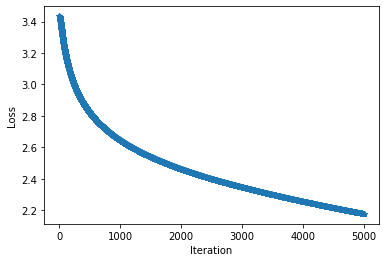
\includegraphics[width=0.6\textwidth,keepaspectratio]{figs/loss_gru.png}
  \label{fig3:gru_loss}
\end{figure}


Apart from complete test-set evaluation, we also analyzed the performance of the various models with a random sample of 3000 unique names. The baseline with 1-NN with edit distance model predicts 58\% of the states correctly, as compared to 95.9\% with our best-performing GRU model. However, in real life the type of inference requests coming in depends on how frequently a name occurs, for this reason, we provide an in-depth comparison of our models across various weighting strategies, as shown in Table \ref{model_comparison}.

\begin{table}
\centering
\caption{Accuracy of Different Models on the Test Set}
\label{model_comparison}
\begin{tabular}{lrrrr}
\toprule
Model & Test Set & Weighted Random (3k) & Top-3k & Bottom-3k \\
\midrule
RNN & 64.8 & 65.5 & 64.6 & 62.0 \\
LSTM & 74.8 & 74.1 & 70.9 & 73.2 \\
GRU & 81.3 & 81.2 & 77.4 & 79.8 \\
\bottomrule
\end{tabular}
\end{table}


\begin{table}
\centering
\caption{Accuracy of Different Models By State of Residence}
\label{accuracy_by_state}
\begin{tabular}{lrrrr}
\toprule
State & 1-NN & RNN & LSTM & GRU \\
\midrule
Andaman & 14.7 & 16.5 & 20.8 & 69.6 \\
Andhra Pradesh & 79.7 & 43.4 & 55.5 & 63.0 \\
Arunachal & 28.3 & 70.2 & 73.6 & 69.0 \\
Assam & 16.7 & 53.1 & 93.6 & 95.3 \\
Bihar & 31.7 & 0.5 & 5.5 & 3.7 \\
Chandigarh & 1.3 & 88.1 & 80.9 & 42.2 \\
Dadra & 28.9 & 44.3 & 71.1 & 73.1 \\
Daman & 12.8 & 21.9 & 42.7 & 62.7 \\
Delhi & 63.9 & 49.9 & 16.8 & 33.6 \\
Goa & 27.8 & 24.6 & 40.1 & 43.9 \\
Gujarat & 86.5 & 74.5 & 88.7 & 90.1 \\
Haryana & 83.0 & 83.4 & 31.0 & 86.1 \\
Jharkhand & 18.9 & 12.0 & 18.0 & 23.6 \\
Jammu and Kashmir & 20.7 & 23.6 & 89.1 & 87.2 \\
Karnataka & 67.8 & 74.0 & 84.1 & 93.2 \\
Kerala & 68.3 & 30.5 & 44.4 & 23.0 \\
Maharashtra & 84.6 & 21.1 & 32.5 & 45.8 \\
Manipur & 63.2 & 13.5 & 37.4 & 45.2 \\
Meghalaya & 48.7 & 51.0 & 78.0 & 76.2 \\
Mizoram & 63.3 & 59.8 & 76.4 & 81.6 \\
Madhya Pradesh & 40.0 & 6.3 & 5.1 & 46.4 \\
Nagaland & 28.5 & 45.4 & 64.0 & 63.4 \\
\bottomrule
\end{tabular}
\end{table}



% TODO: Find the right place for this
We split the data by last names, which keeps the last names distinct between the two sets. We keep 80\% of the data for training and 20\% for testing. On the test set, the top-3 accuracy—-chances that our three predictions include the modal state in which people with that last name live—of our model is 81.3\%. Compare this to the no-information baseline where we only know the states' population and guess the modal state. The most populous state in India is Uttar Pradesh and if we were to guess that as the answer for all the names, we would be right less than 16.74\% of the time. The 1-NN with edit distance results can be seen as another baseline but as we write above, we believe the 1-NN results reflect the fact that there is a quasi-overlap between training and test sets. Technically, the overlap should help with the RNN though our RNN is shallow and cannot learn very complex patterns. 

\section{States to Languages}

To create our states to languages database, we consulted the state constitutions for the official languages and the latest Indian census (the 2011 census) for the most widely spoken languages in the state. We then append the mapping to our state predictions. Our method has some weaknesses. While the modern Indian state boundaries and state education curricula are affected by language conflicts (for instance, there were \href{https://en.wikipedia.org/wiki/Anti-Hindi_agitations_of_Tamil_Nadu}{anti-Hindi agitations in Tamil Nadu}), there is no unique mapping between states and languages. This is for a few reasons. For one, many Indian states are massive and there is considerable linguistic diversity across regions within states. Second, internal migration, especially to urban centers, has transformed many cities. For instance, say that all Dhingras only speak Punjabi and say that all of them once upon a time lived in Punjab. Suppose that over time half of them immigrated to Delhi and never learned another language. Say that we map Delhi to people who understand Hindi. Our classifier will then indicate that Dhingras have a 50\% chance of speaking Punjabi and a 50\% chance of speaking Hindi. But in fact, no Dhingra can understand Hindi. Our prediction in such a case would be highly erroneous. We have reasons to think, however, that the net error is generally likely lower. For instance, in the above example, we make the slightly untenable assumption that immigrants never learn to understand the dominant language of the geography they immigrate to. This can be true but it is also likely that there is both selection bias—Dhingras who are open to learning new languages or may already know another language are likelier to immigrate to Delhi—and learning—Dhingras who immigrate to Delhi learn a new language over time. The other compensating virtue of our dataset, as we noted above, is that electoral rolls still map immigrants to their home districts. To the extent that immigrants do not forget their mother tongue, we will have good predictions. 

\section{Discussion}

Our paper contributes to technologies that improve localization. However, our method of predicting languages understood by the user from their last name has a few limitations. The first is that our geographical units are very crude. Indian states are often as big as countries. For instance, Uttar Pradesh has more than 230 million people. There is also a large linguistic diversity within the states. In future versions, we hope to exploit the more granular data provided in the electoral rolls. Second, the relationship between geography and language is weaker because of internal migration. This is especially true in urban areas. Though as we note, our unique database of electoral rolls has the virtue of mapping people to their home districts. The third challenge is transliteration. There is no one standard way of transliterating Indian languages into English. We use one transliteration when the way to improve coverage may be to use k-best transliterations with the transliterations produced roughly in the frequency of how common they are. The fourth challenge is establishing last names. Our method of establishing the last name is crude. One way to improve the heuristic is to only use last words in names that are common across household members’ names. 

\newpage

\bibliography{instate.bib}

\end{document}